\section{ Results}
\label{sec:results}

\subsection{The Gate Reproduces Its Specification}
\label{sec:conformance}
Under the authored labels the gate permits 259 of the 2,520 flows and denies
2,261, matching the expected result of Table~\ref{tab:flows} on every flow.
There are no false permits and no false denials, and the result holds within
each of the six flow classes and each of the six realized sensitivity tiers.
This confirms the gate was built correctly, so every failure reported below
originates in a label.

\subsection{Substituting the Annotator}
\label{sec:substitution-results}
Table~\ref{tab:conformance} reports what happens when a model supplies the
labels instead. Every configuration degrades the enforced policy: between 9 and
64 flows that the authored policy denies are released, and between 26 and 100
that it permits are refused.

\begin{table}[t]
\centering
\caption{Label conformance against the authored policy. Tier and ACL are the
share of the 105 documents labeled exactly as authored. PV and OB are induced
privacy violations and over-blocks out of 2,520 flows. O:U is the ratio of
over-granted to under-granted roles.}
\label{tab:conformance}
\footnotesize
\setlength{\tabcolsep}{4pt}
\resizebox{0.58\columnwidth}{!}{%
\begin{tabular}{@{}lrrrrr@{}}
\toprule
\textbf{Configuration} & \textbf{Tier} & \textbf{ACL} & \textbf{PV} & \textbf{OB} & \textbf{O:U} \\
\midrule
Opus 4.8            & 78\% & 55\% & 40 &  31 & 2.29 \\
Opus 4.8 (no think) & 83\% & 57\% & 44 &  27 & 2.16 \\
Sonnet 5            & 82\% & 52\% & 64 &  34 & 2.04 \\
Haiku 4.5           & 84\% & 30\% & 39 &  28 & 4.45 \\
\addlinespace
GPT-5.4             & 86\% & 23\% &  9 & 100 & 1.38 \\
GPT-5.4-mini        & 83\% & 80\% & 11 &  26 & 0.68 \\
GPT-5.4-nano        & 82\% & 69\% & 16 &  36 & 1.23 \\
\bottomrule
\end{tabular}}
\end{table}

The two label fields do not fail equally. Tier conformance is high and tightly
clustered, from 78\% to 86\% across all seven configurations and both
providers. ACL conformance ranges from 23\% to 80\%. This asymmetry is the
central empirical fact of our study. The tier is the field a document's type
nearly determines (Section~\ref{sec:substitution}); the ACL records a decision
the document's contents do not determine. Counterfactual flip-back
(Section~\ref{sec:attribution}) attributes every induced violation to
\texttt{permitted\_receiver\_roles}.

\begin{figure}[t]
  \centering
  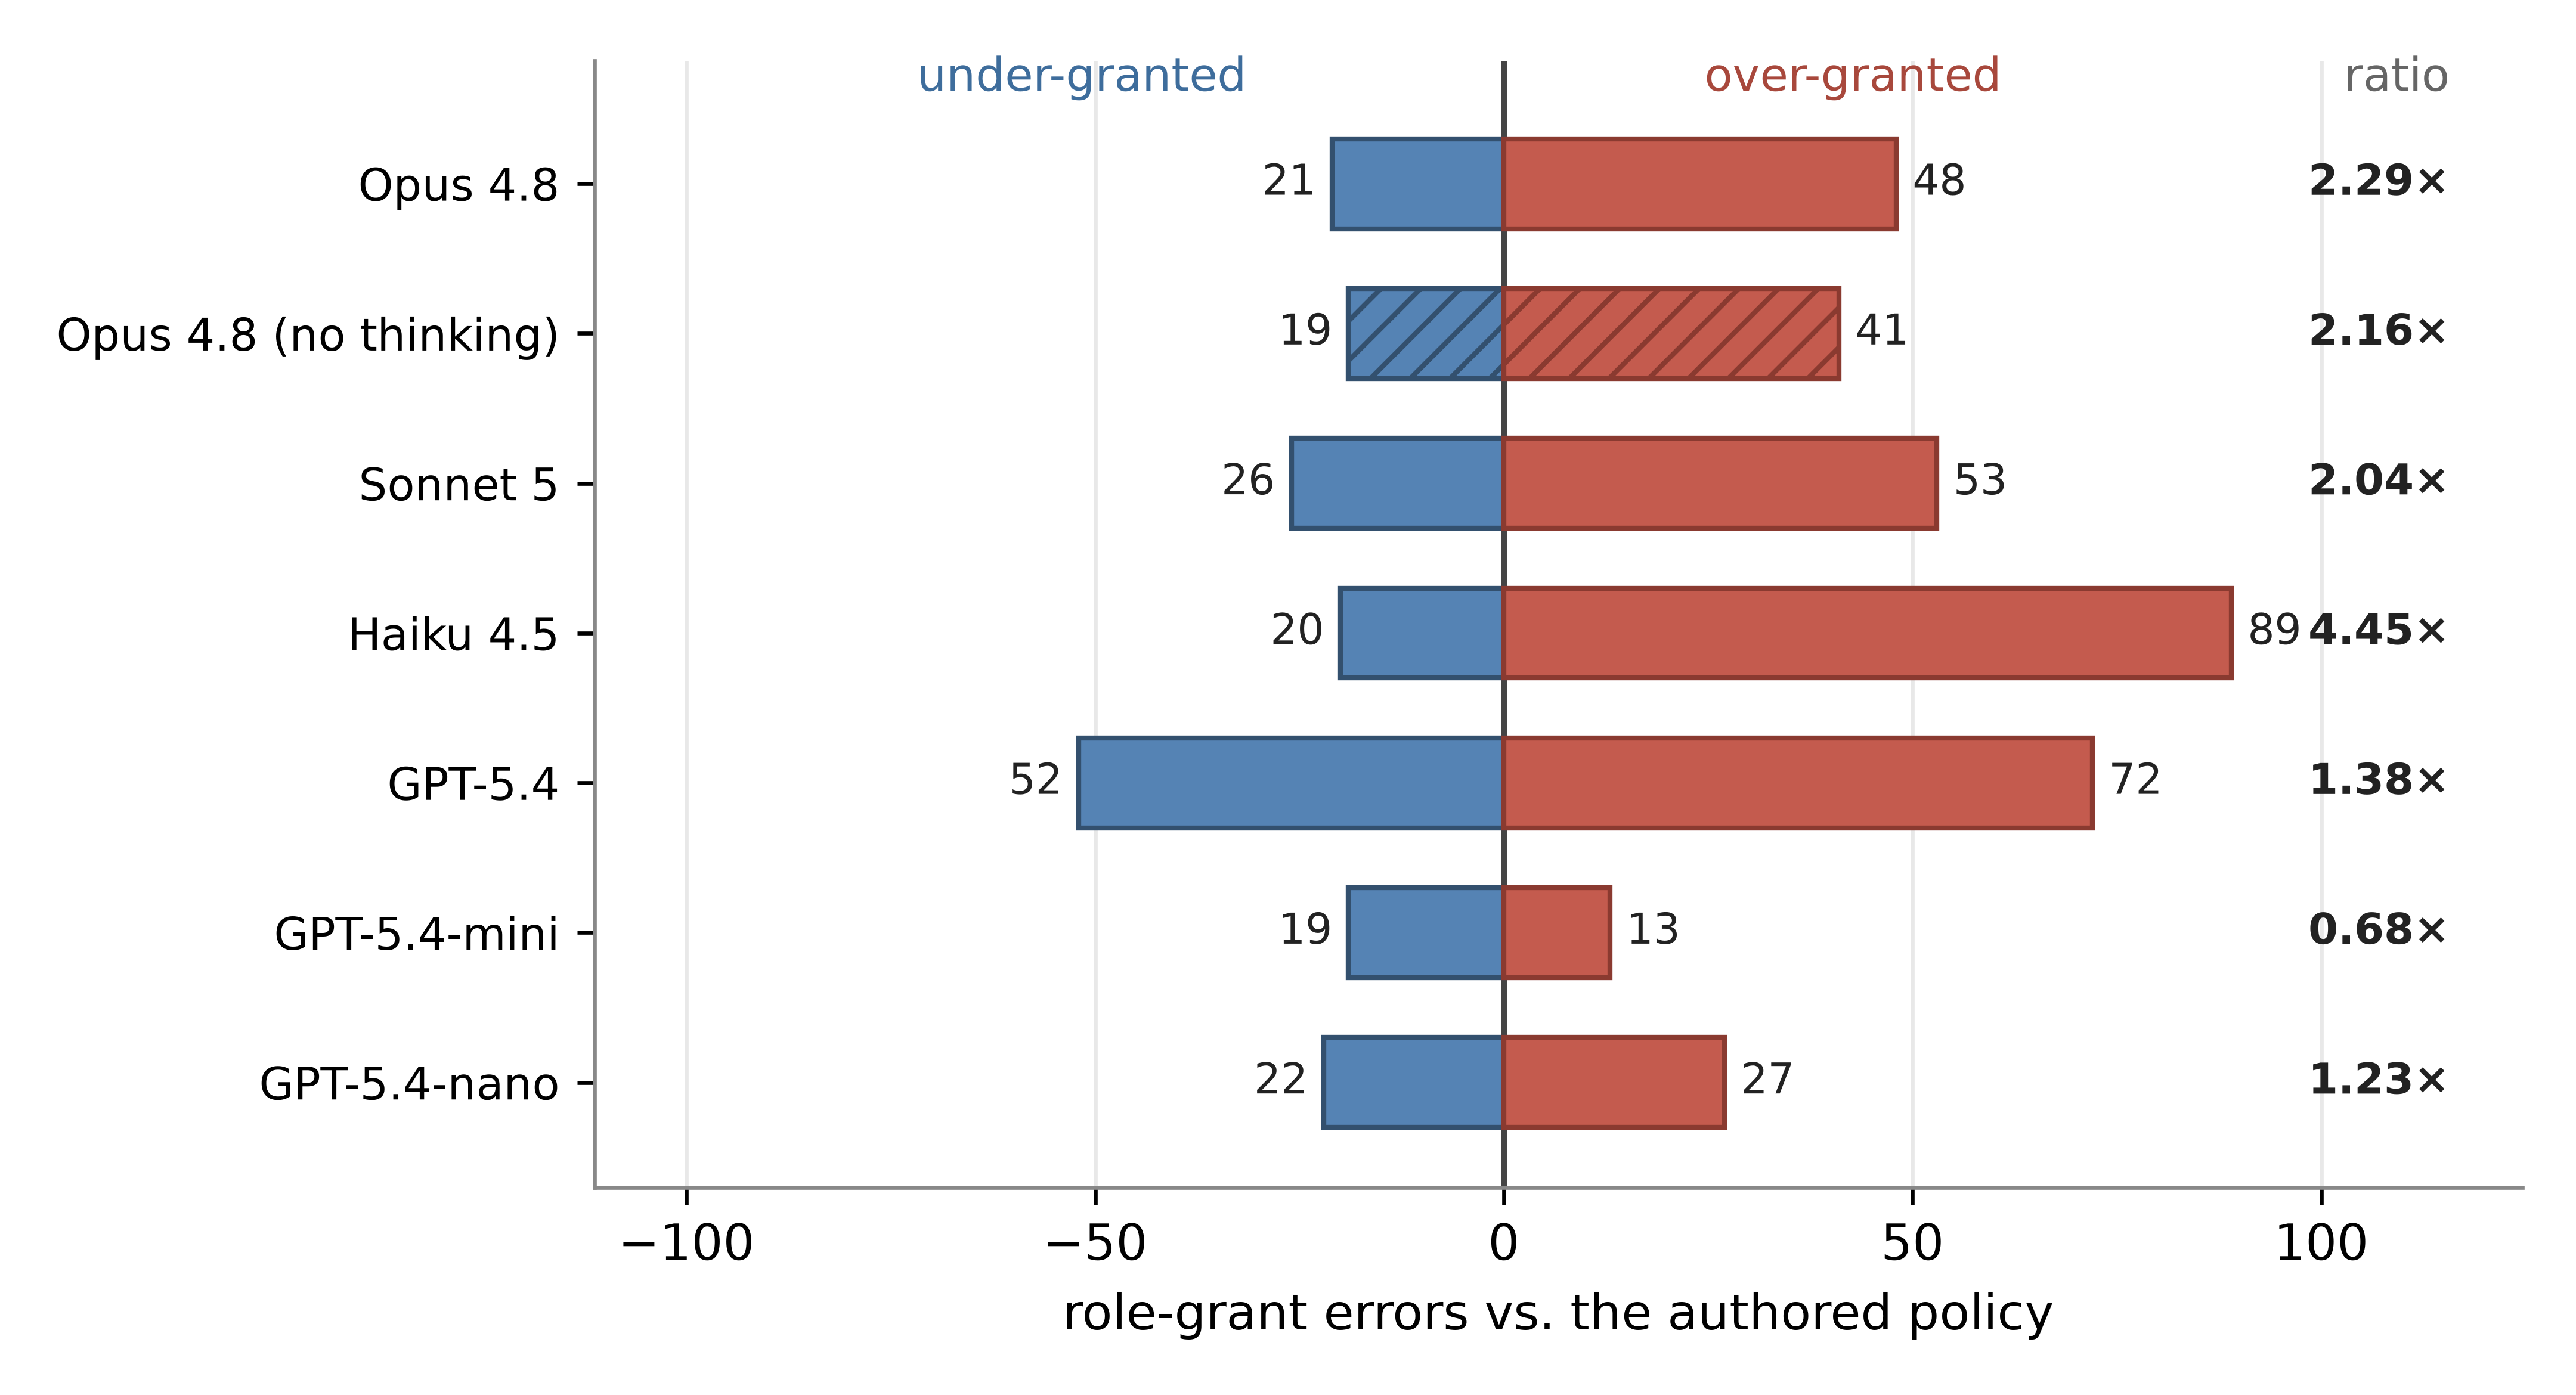
\includegraphics[width=0.93\columnwidth]{figures/x2_direction}
  \caption{Direction of role-grant error against the authored policy.
  \textit{Over-granting} releases records the policy withholds;
  \textit{under-granting} withholds records it permits.}
  \label{fig:direction}
\end{figure}

Figure~\ref{fig:direction} shows the direction of the error. Anthropic
configurations grant roles the policy withholds at 2.04 to 4.45 times the rate
at which they withhold roles it grants; {\em Haiku 4.5} is the most permissive
at 4.45$\times$. The OpenAI configurations are less permissive, from
1.38$\times$ down to 0.68$\times$, with {\em GPT-5.4-mini} the only
configuration that errs toward refusal. Different models therefore carry
different authorization biases, which makes model selection itself a
privacy-policy decision wherever a model authors the policy.

Neither direction is safe. {\em GPT-5.4} has both the highest tier conformance
(86\%) and the lowest ACL conformance (23\%), and it produces the fewest
privacy violations (9) together with by far the most over-blocks (100). A
system that refuses 100 legitimate requests has failed its users.

\subsection{Models Do Not Agree With Themselves}
\label{sec:selfconsistency}
Table~\ref{tab:selfconsistency} compares each configuration's five draws to
one another, every draw a relabeling of the same 105 documents under an
identical request.

\begin{table}[t]
\centering
\caption{Self-consistency across five draws. Tier, ACL, and All report the fraction of 105 documents with unanimous agreement across all draws. Unstable counts decisions that vary across draws; UUD denotes the subset denied by the authored policy.}
\label{tab:selfconsistency}
\footnotesize
\setlength{\tabcolsep}{4pt}
\resizebox{0.64\columnwidth}{!}{%
\begin{tabular}{@{}lrrrrr@{}}
\toprule
\textbf{Configuration} & \textbf{Tier} & \textbf{ACL} & \textbf{All} & \textbf{Unstable} & \textbf{UUD} \\
\midrule
Opus 4.8            & 93\% & 56\% & 52\% & 115 & 66 \\
Opus 4.8 (no think) & 97\% & 62\% & 59\% & 108 & 73 \\
Sonnet 5            & 97\% & 63\% & 62\% &  96 & 68 \\
Haiku 4.5           & 87\% & 26\% & 26\% & 124 & 62 \\
\addlinespace
GPT-5.4             & 99\% & 76\% & 76\% &  40 &  0 \\
GPT-5.4-mini        & 90\% & 90\% & 83\% &  28 &  2 \\
GPT-5.4-nano        & 99\% & 91\% & 88\% &  13 &  9 \\
\bottomrule
\end{tabular}
}
\end{table}

No configuration is stable, and the asymmetry seen in conformance reappears
more sharply: every configuration reproduces its own tier on 87\% to 99\% of
documents but its own ACL on as little as 26\%. The provider bands do not
overlap: Anthropic configurations reproduce the ACL on 26--63\% of documents,
OpenAI on 76--91\%. This gap is confounded with sampling, since the Anthropic
configurations ran at default settings (Section~\ref{sec:models}); the OpenAI
configurations, run at temperature 0 where permitted, are still unstable.

The consequences appear at the decision layer. Between 13 and 124 of the 2,520
access decisions change between draws with no change to any input.
Table~\ref{tab:perdraw} gives the per-draw counts: {\em Opus 4.8} induces
between 34 and 57 privacy violations depending only on which draw is consulted,
and {\em Sonnet 5} between 46 and 64.

\begin{table}[!t]
\centering
\caption{Induced privacy violations per draw, adjudicated by the same gate. Draw 1 is the single-draw result reported in Table~\ref{tab:conformance}.}
\label{tab:perdraw}
\footnotesize
\resizebox{0.91\linewidth}{!}{%
\begin{tabular}{@{}lrrrrrrrr@{}}
\toprule
\textbf{Configuration} & \textbf{Draw 1} & \textbf{Draw 2} & \textbf{Draw 3} &
\textbf{Draw 4} & \textbf{Draw 5} & \textbf{Min} & \textbf{Max} & \textbf{Range} \\
\midrule
Opus 4.8            & 40 & 43 & 57 & 52 & 34 & 34 & 57 & 23 \\
Opus 4.8 (no think) & 44 & 52 & 32 & 21 & 23 & 21 & 52 & 31 \\
Sonnet 5            & 64 & 56 & 63 & 46 & 56 & 46 & 64 & 18 \\
Haiku 4.5           & 39 & 38 & 39 & 26 & 25 & 25 & 39 & 14 \\
\addlinespace
GPT-5.4             &  9 &  9 &  9 &  9 &  9 &  9 &  9 &  0 \\
GPT-5.4-mini        & 11 & 10 & 11 & 12 & 10 & 10 & 12 &  2 \\
GPT-5.4-nano        & 16 & 17 & 13 & 13 & 16 & 13 & 17 &  4 \\
\bottomrule
\end{tabular}
}
\end{table}

\begin{figure*}[!t]
  \centering
  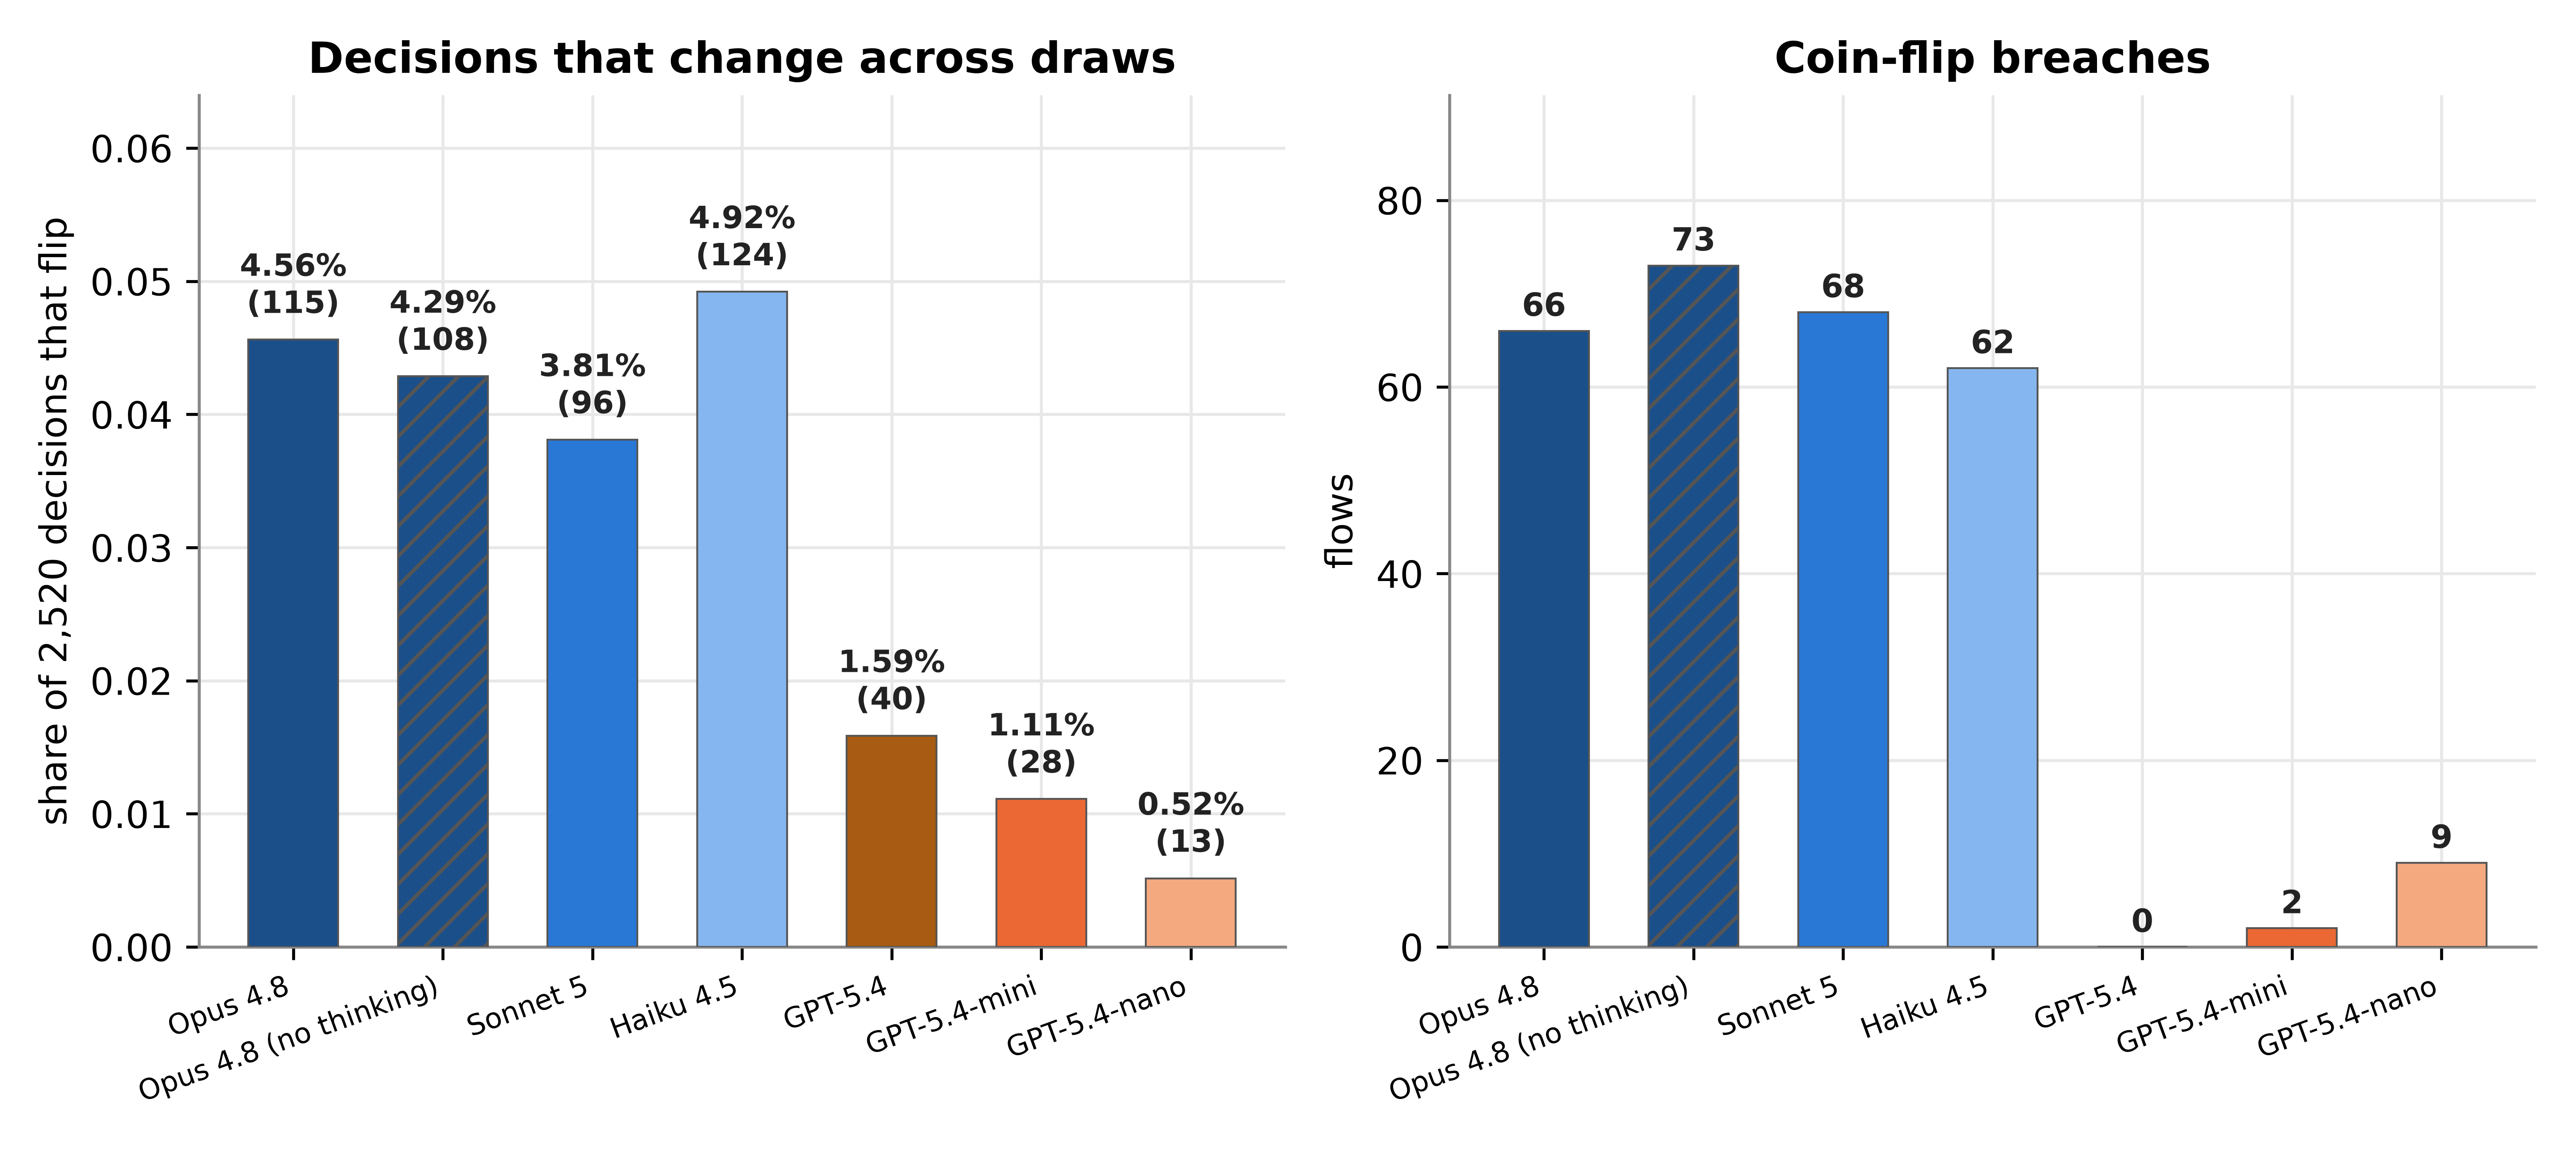
\includegraphics[width=0.68\linewidth]{figures/x5_instability}
  \caption{(a) \textbf{Left:} share of the 2,520 access decisions that change
  between draws. (b) \textbf{Right:} the subset the authored policy denies, where a
  re-roll decides whether the record is released. The two panels are not
  proportional.}
  \label{fig:instability}
\end{figure*}

The count of unstable decisions understates the risk, because it does not show
which decisions move (Fig.~\ref{fig:instability}). Anthropic configurations
carry 62 to 73 unstable unauthorized disclosures; the OpenAI configurations
carry 0 to 9. {\em GPT-5.4} is the limiting case in one direction, with 40
unstable flows and none on denied flows: it is erratic but never newly
disclosive. {\em GPT-5.4-nano} is the limiting case in the other: the most
self-consistent configuration, with only 13 unstable flows, yet 69\% of them
fall on denied flows. Stability and safety are separate properties, and a
single aggregate of either will mislead.

\subsection{Controls}
\label{sec:controls}
Tier conformance is not uniform across tiers. Every configuration reproduces
the authored tier on all or nearly all documents in the \texttt{employment},
\texttt{clinical\_sensitive}, \texttt{internal}, and \texttt{public} tiers,
while conformance on \texttt{clinical\_standard} ranges from 59\% to 79\% and
on \texttt{financial} from 48\% to 88\%. Those two tiers hold 64 of the 105
documents, so the gross rate of 78\% to 86\% is a composition effect: a
generation cue carried in the content would raise conformance uniformly, and it
does not. The residual error concentrates where content underdetermines the
boundary, on records carrying both clinical and financial material. Any
remaining cue can only raise conformance, so it cannot explain the ACL
failures.

Inverting \texttt{extra\_sensitive} on all 105 documents and re-adjudicating
leaves all 2,520 decisions unchanged, with permits fixed at 259. The field is
inert at the gate, as Table~\ref{tab:label-fields} records. We exhibit that aggregation does not recover what a single draw loses. A five-draw majority vote yields 33 induced violations for {\em Opus 4.8}, or 1.5\% of the 2,261 flows the policy denies. That is barely below its single-draw range of 34--57 (1.5--2.5\%). For {\em Sonnet 5}, it yields 66
(2.9\%), more than any of the five draws it aggregates (46--64, or 2.0-2.8\%). %\footnote{\color{green!50!black}contextualize these numebrs on \% context. \textbf{[Done]}}

\subsection{External Policy Authority}
\label{sec:privaci-results}
On the 214 PrivaCI-Bench flows, the most accurate configuration,
{\em GPT-5.4-mini}, matches the court-grounded label on 87.8\% of flows. Only
20 flows are prohibited, so overall accuracy is dominated by flows that HIPAA
permits or does not govern. Of those 20, {\em GPT-5.4-mini} labels 11 as
permitted.
